\documentclass[]{article}
\usepackage{lmodern}
\usepackage{amssymb,amsmath}
\usepackage{ifxetex,ifluatex}
\usepackage{fixltx2e} % provides \textsubscript
\ifnum 0\ifxetex 1\fi\ifluatex 1\fi=0 % if pdftex
  \usepackage[T1]{fontenc}
  \usepackage[utf8]{inputenc}
\else % if luatex or xelatex
  \ifxetex
    \usepackage{mathspec}
  \else
    \usepackage{fontspec}
  \fi
  \defaultfontfeatures{Ligatures=TeX,Scale=MatchLowercase}
\fi
% use upquote if available, for straight quotes in verbatim environments
\IfFileExists{upquote.sty}{\usepackage{upquote}}{}
% use microtype if available
\IfFileExists{microtype.sty}{%
\usepackage{microtype}
\UseMicrotypeSet[protrusion]{basicmath} % disable protrusion for tt fonts
}{}
\usepackage[margin=1in]{geometry}
\usepackage{hyperref}
\hypersetup{unicode=true,
            pdftitle={HW3:~Logistic~Regression},
            pdfauthor={Ebeid ElSayed - Ebeid@gatech.edu},
            pdfborder={0 0 0},
            breaklinks=true}
\urlstyle{same}  % don't use monospace font for urls
\usepackage{color}
\usepackage{fancyvrb}
\newcommand{\VerbBar}{|}
\newcommand{\VERB}{\Verb[commandchars=\\\{\}]}
\DefineVerbatimEnvironment{Highlighting}{Verbatim}{commandchars=\\\{\}}
% Add ',fontsize=\small' for more characters per line
\usepackage{framed}
\definecolor{shadecolor}{RGB}{248,248,248}
\newenvironment{Shaded}{\begin{snugshade}}{\end{snugshade}}
\newcommand{\KeywordTok}[1]{\textcolor[rgb]{0.13,0.29,0.53}{\textbf{{#1}}}}
\newcommand{\DataTypeTok}[1]{\textcolor[rgb]{0.13,0.29,0.53}{{#1}}}
\newcommand{\DecValTok}[1]{\textcolor[rgb]{0.00,0.00,0.81}{{#1}}}
\newcommand{\BaseNTok}[1]{\textcolor[rgb]{0.00,0.00,0.81}{{#1}}}
\newcommand{\FloatTok}[1]{\textcolor[rgb]{0.00,0.00,0.81}{{#1}}}
\newcommand{\ConstantTok}[1]{\textcolor[rgb]{0.00,0.00,0.00}{{#1}}}
\newcommand{\CharTok}[1]{\textcolor[rgb]{0.31,0.60,0.02}{{#1}}}
\newcommand{\SpecialCharTok}[1]{\textcolor[rgb]{0.00,0.00,0.00}{{#1}}}
\newcommand{\StringTok}[1]{\textcolor[rgb]{0.31,0.60,0.02}{{#1}}}
\newcommand{\VerbatimStringTok}[1]{\textcolor[rgb]{0.31,0.60,0.02}{{#1}}}
\newcommand{\SpecialStringTok}[1]{\textcolor[rgb]{0.31,0.60,0.02}{{#1}}}
\newcommand{\ImportTok}[1]{{#1}}
\newcommand{\CommentTok}[1]{\textcolor[rgb]{0.56,0.35,0.01}{\textit{{#1}}}}
\newcommand{\DocumentationTok}[1]{\textcolor[rgb]{0.56,0.35,0.01}{\textbf{\textit{{#1}}}}}
\newcommand{\AnnotationTok}[1]{\textcolor[rgb]{0.56,0.35,0.01}{\textbf{\textit{{#1}}}}}
\newcommand{\CommentVarTok}[1]{\textcolor[rgb]{0.56,0.35,0.01}{\textbf{\textit{{#1}}}}}
\newcommand{\OtherTok}[1]{\textcolor[rgb]{0.56,0.35,0.01}{{#1}}}
\newcommand{\FunctionTok}[1]{\textcolor[rgb]{0.00,0.00,0.00}{{#1}}}
\newcommand{\VariableTok}[1]{\textcolor[rgb]{0.00,0.00,0.00}{{#1}}}
\newcommand{\ControlFlowTok}[1]{\textcolor[rgb]{0.13,0.29,0.53}{\textbf{{#1}}}}
\newcommand{\OperatorTok}[1]{\textcolor[rgb]{0.81,0.36,0.00}{\textbf{{#1}}}}
\newcommand{\BuiltInTok}[1]{{#1}}
\newcommand{\ExtensionTok}[1]{{#1}}
\newcommand{\PreprocessorTok}[1]{\textcolor[rgb]{0.56,0.35,0.01}{\textit{{#1}}}}
\newcommand{\AttributeTok}[1]{\textcolor[rgb]{0.77,0.63,0.00}{{#1}}}
\newcommand{\RegionMarkerTok}[1]{{#1}}
\newcommand{\InformationTok}[1]{\textcolor[rgb]{0.56,0.35,0.01}{\textbf{\textit{{#1}}}}}
\newcommand{\WarningTok}[1]{\textcolor[rgb]{0.56,0.35,0.01}{\textbf{\textit{{#1}}}}}
\newcommand{\AlertTok}[1]{\textcolor[rgb]{0.94,0.16,0.16}{{#1}}}
\newcommand{\ErrorTok}[1]{\textcolor[rgb]{0.64,0.00,0.00}{\textbf{{#1}}}}
\newcommand{\NormalTok}[1]{{#1}}
\usepackage{graphicx,grffile}
\makeatletter
\def\maxwidth{\ifdim\Gin@nat@width>\linewidth\linewidth\else\Gin@nat@width\fi}
\def\maxheight{\ifdim\Gin@nat@height>\textheight\textheight\else\Gin@nat@height\fi}
\makeatother
% Scale images if necessary, so that they will not overflow the page
% margins by default, and it is still possible to overwrite the defaults
% using explicit options in \includegraphics[width, height, ...]{}
\setkeys{Gin}{width=\maxwidth,height=\maxheight,keepaspectratio}
\IfFileExists{parskip.sty}{%
\usepackage{parskip}
}{% else
\setlength{\parindent}{0pt}
\setlength{\parskip}{6pt plus 2pt minus 1pt}
}
\setlength{\emergencystretch}{3em}  % prevent overfull lines
\providecommand{\tightlist}{%
  \setlength{\itemsep}{0pt}\setlength{\parskip}{0pt}}
\setcounter{secnumdepth}{0}
% Redefines (sub)paragraphs to behave more like sections
\ifx\paragraph\undefined\else
\let\oldparagraph\paragraph
\renewcommand{\paragraph}[1]{\oldparagraph{#1}\mbox{}}
\fi
\ifx\subparagraph\undefined\else
\let\oldsubparagraph\subparagraph
\renewcommand{\subparagraph}[1]{\oldsubparagraph{#1}\mbox{}}
\fi

%%% Use protect on footnotes to avoid problems with footnotes in titles
\let\rmarkdownfootnote\footnote%
\def\footnote{\protect\rmarkdownfootnote}

%%% Change title format to be more compact
\usepackage{titling}

% Create subtitle command for use in maketitle
\newcommand{\subtitle}[1]{
  \posttitle{
    \begin{center}\large#1\end{center}
    }
}

\setlength{\droptitle}{-2em}
  \title{HW3:~Logistic~Regression}
  \pretitle{\vspace{\droptitle}\centering\huge}
  \posttitle{\par}
\subtitle{CSE6242 - Data and Visual Analytics - Spring 2017}
  \author{Ebeid ElSayed -
\href{mailto:Ebeid@gatech.edu}{\nolinkurl{Ebeid@gatech.edu}}}
  \preauthor{\centering\large\emph}
  \postauthor{\par}
  \predate{\centering\large\emph}
  \postdate{\par}
  \date{March 14, 2017}

\usepackage{docmute}

\begin{document}
\maketitle

\begin{Shaded}
\begin{Highlighting}[]
\KeywordTok{setwd}\NormalTok{(}\StringTok{"C:/Users/eelsayed/Google Drive/CSE 6242/2017 Spring"}\NormalTok{)}
\end{Highlighting}
\end{Shaded}

\subsection{0. Data Preprocessing}\label{data-preprocessing}

0.a \& 0.b

\begin{Shaded}
\begin{Highlighting}[]
\NormalTok{rawDatalLoaded <-}\StringTok{ }\OtherTok{TRUE}

\NormalTok{if(}\KeywordTok{file.exists}\NormalTok{(}\StringTok{"mnist_train.csv"}\NormalTok{))\{}
  \NormalTok{train <-}\StringTok{ }\KeywordTok{read.csv}\NormalTok{(}\DataTypeTok{file=}\StringTok{"mnist_train.csv"}\NormalTok{, }\DataTypeTok{header =} \OtherTok{FALSE}\NormalTok{)}
\NormalTok{\}else\{}
  \NormalTok{rawDatalLoaded <-}\StringTok{ }\OtherTok{FALSE}
\NormalTok{\}}

\NormalTok{if(}\KeywordTok{file.exists}\NormalTok{(}\StringTok{"mnist_test.csv"}\NormalTok{))\{}
  \NormalTok{test <-}\StringTok{ }\KeywordTok{read.csv}\NormalTok{(}\DataTypeTok{file=}\StringTok{"mnist_test.csv"}\NormalTok{, }\DataTypeTok{header =} \OtherTok{FALSE}\NormalTok{)}
\NormalTok{\}else\{}
  \NormalTok{rawDatalLoaded <-}\StringTok{ }\OtherTok{FALSE}
\NormalTok{\}}

\NormalTok{if(!rawDatalLoaded)\{}
  \KeywordTok{print}\NormalTok{(}\StringTok{"Data wasn't loaded correctly."}\NormalTok{)}
\NormalTok{\}}

\NormalTok{train <-}\StringTok{ }\KeywordTok{as.data.frame}\NormalTok{(}\KeywordTok{t}\NormalTok{(train))}
\KeywordTok{names}\NormalTok{(train)[}\DecValTok{785}\NormalTok{] <-}\StringTok{ "Label"}

\NormalTok{test <-}\StringTok{ }\KeywordTok{as.data.frame}\NormalTok{(}\KeywordTok{t}\NormalTok{(test))}
\KeywordTok{names}\NormalTok{(test)[}\DecValTok{785}\NormalTok{] <-}\StringTok{ "Label"}
\end{Highlighting}
\end{Shaded}

0.c Partition~the training set for classification of 0, 1 and 3, 5
classes based on the class label (last row 785): train\_0\_1,
train\_3\_5.

\begin{Shaded}
\begin{Highlighting}[]
\NormalTok{train_0_1 <-}\StringTok{ }\NormalTok{train[(train$Label ==}\StringTok{ }\DecValTok{0}\NormalTok{) |}\StringTok{ }\NormalTok{(train$Label ==}\StringTok{ }\DecValTok{1}\NormalTok{),]}
\NormalTok{train_3_5 <-}\StringTok{ }\NormalTok{train[(train$Label ==}\StringTok{ }\DecValTok{3}\NormalTok{) |}\StringTok{ }\NormalTok{(train$Label ==}\StringTok{ }\DecValTok{5}\NormalTok{),]}
\end{Highlighting}
\end{Shaded}

0.d Do the same for the test set: test\_0\_1, test\_3\_5.

\begin{Shaded}
\begin{Highlighting}[]
\NormalTok{test_0_1 <-}\StringTok{ }\NormalTok{test[(test$Label ==}\StringTok{ }\DecValTok{0}\NormalTok{) |}\StringTok{ }\NormalTok{(test$Label ==}\StringTok{ }\DecValTok{1}\NormalTok{),]}
\NormalTok{test_3_5 <-}\StringTok{ }\NormalTok{test[(test$Label ==}\StringTok{ }\DecValTok{3}\NormalTok{) |}\StringTok{ }\NormalTok{(test$Label ==}\StringTok{ }\DecValTok{5}\NormalTok{),]}
\end{Highlighting}
\end{Shaded}

0.e \& 0.f \textbar{} Separate the class label from all the partitions
created (remove row 785 from the actual data and store it as a separate
vector).

\begin{Shaded}
\begin{Highlighting}[]
\NormalTok{true_label_train_0_1 <-}\StringTok{ }\NormalTok{train_0_1$Label}
\NormalTok{train_0_1 <-}\StringTok{ }\KeywordTok{subset}\NormalTok{(train_0_1, }\DataTypeTok{select =} \KeywordTok{names}\NormalTok{(train_0_1) !=}\StringTok{ "Label"} \NormalTok{)}

\NormalTok{true_label_train_3_5 <-}\StringTok{ }\NormalTok{train_3_5$Label}
\NormalTok{train_3_5 <-}\StringTok{ }\KeywordTok{subset}\NormalTok{(train_3_5, }\DataTypeTok{select =} \KeywordTok{names}\NormalTok{(train_3_5) !=}\StringTok{ "Label"} \NormalTok{)}

\NormalTok{true_label_test_0_1 <-}\StringTok{ }\NormalTok{test_0_1$Label}
\NormalTok{test_0_1 <-}\StringTok{ }\KeywordTok{subset}\NormalTok{(test_0_1, }\DataTypeTok{select =} \KeywordTok{names}\NormalTok{(test_0_1) !=}\StringTok{ "Label"} \NormalTok{)}

\NormalTok{true_label_test_3_5 <-}\StringTok{ }\NormalTok{test_3_5$Label}
\NormalTok{test_3_5 <-}\StringTok{ }\KeywordTok{subset}\NormalTok{(test_3_5, }\DataTypeTok{select =} \KeywordTok{names}\NormalTok{(test_3_5) !=}\StringTok{ "Label"} \NormalTok{)}
\end{Highlighting}
\end{Shaded}

0.g Visualize 1 image from each class to ensure you have read in the
data correctly. You will have 4 images corresponding to 0, 1, 3 and 5.
You need to convert the 1D image data into 2D for visualisation.

\begin{Shaded}
\begin{Highlighting}[]
\NormalTok{show_digit_image <-}\StringTok{ }\NormalTok{function(df, digitClass, imageTitle) \{}
  \NormalTok{tmp <-}\StringTok{ }\NormalTok{df[df$Label ==}\StringTok{ }\NormalTok{digitClass,]}
  \NormalTok{m <-}\StringTok{ }\KeywordTok{matrix}\NormalTok{(}\KeywordTok{unlist}\NormalTok{(tmp[}\DecValTok{1}\NormalTok{,}\DecValTok{1}\NormalTok{:}\DecValTok{784}\NormalTok{]), }\DataTypeTok{ncol =} \DecValTok{28}\NormalTok{, }\DataTypeTok{byrow =} \OtherTok{TRUE}\NormalTok{)}
  \KeywordTok{image}\NormalTok{(}\DataTypeTok{z =} \NormalTok{m, }\DataTypeTok{col =} \KeywordTok{gray.colors}\NormalTok{(}\DecValTok{256}\NormalTok{))}
  \KeywordTok{title}\NormalTok{(}\DataTypeTok{main =} \NormalTok{imageTitle)}
\NormalTok{\}}
\end{Highlighting}
\end{Shaded}

\begin{Shaded}
\begin{Highlighting}[]
\KeywordTok{show_digit_image}\NormalTok{(train, }\DecValTok{0}\NormalTok{, }\StringTok{"Class label : 0"}\NormalTok{)}
\end{Highlighting}
\end{Shaded}

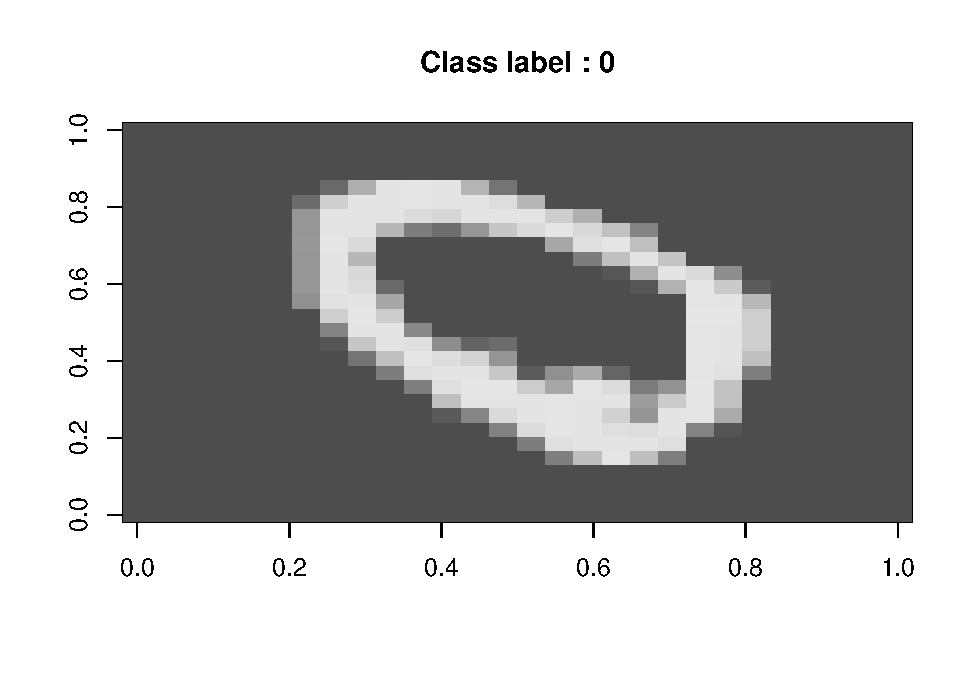
\includegraphics{hw3_files/figure-latex/unnamed-chunk-6-1.pdf}

\begin{Shaded}
\begin{Highlighting}[]
\KeywordTok{show_digit_image}\NormalTok{(train, }\DecValTok{1}\NormalTok{, }\StringTok{"Class label : 1"}\NormalTok{)}
\end{Highlighting}
\end{Shaded}

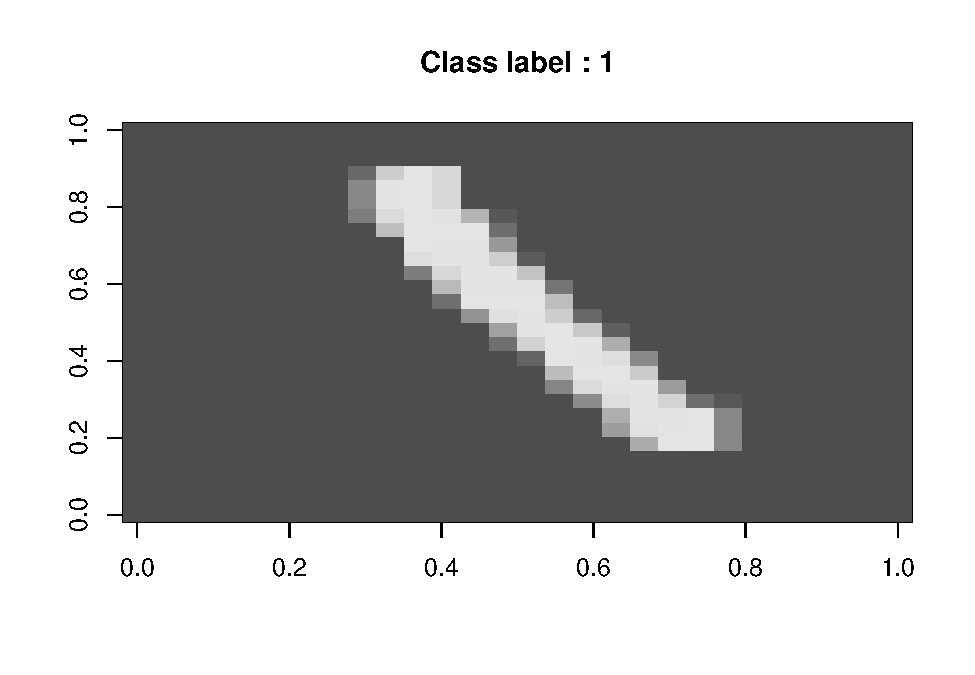
\includegraphics{hw3_files/figure-latex/unnamed-chunk-7-1.pdf}

\begin{Shaded}
\begin{Highlighting}[]
\KeywordTok{show_digit_image}\NormalTok{(train, }\DecValTok{3}\NormalTok{, }\StringTok{"Class label : 3"}\NormalTok{)}
\end{Highlighting}
\end{Shaded}

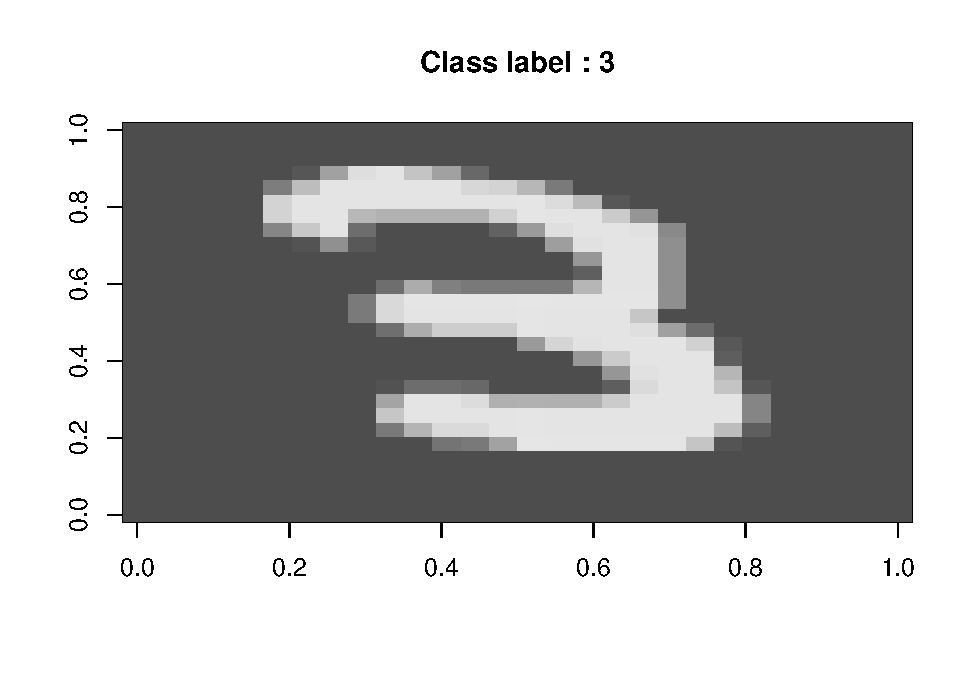
\includegraphics{hw3_files/figure-latex/unnamed-chunk-8-1.pdf}

\begin{Shaded}
\begin{Highlighting}[]
\KeywordTok{show_digit_image}\NormalTok{(train, }\DecValTok{5}\NormalTok{, }\StringTok{"Class label : 5"}\NormalTok{)}
\end{Highlighting}
\end{Shaded}

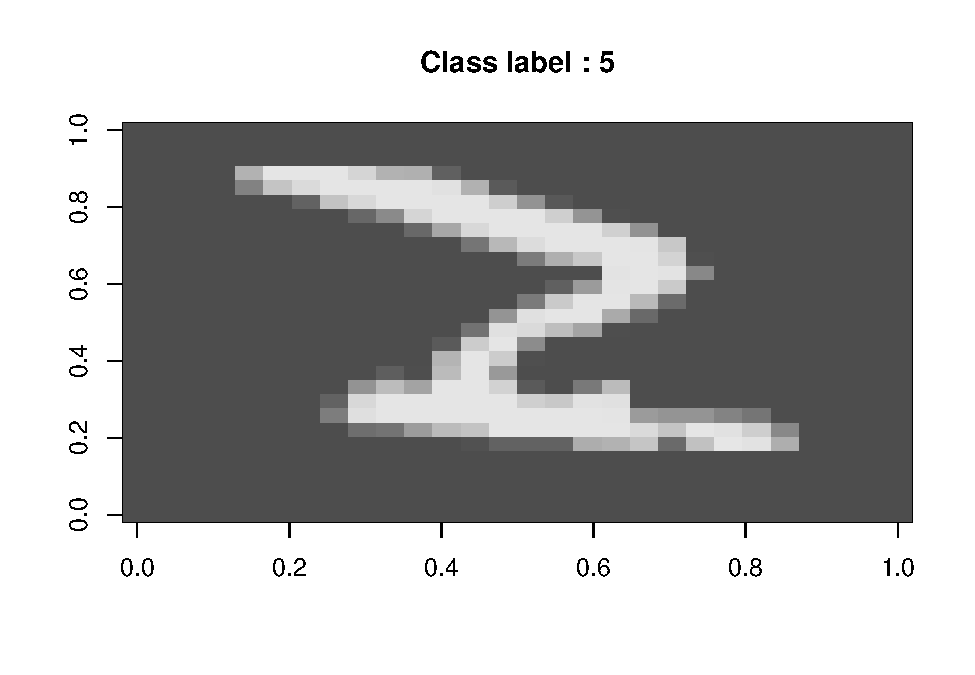
\includegraphics{hw3_files/figure-latex/unnamed-chunk-9-1.pdf}

\subsection{1. Theory}\label{theory}

1.a Write down the formula for computing the gradient of the loss
function used in Logistic Regression. Specify what each variable
represents in the equation.

The formula for the gradient descent is: \[
\theta_j \leftarrow \theta_j - \alpha \sum_{i=1}^{n} \frac{1}{1 + \exp(-y^{(i)} <\theta, x^{(i)}> )}
\] where \(x^{(i)}\) is the data point represented in a vector of
features, \(y^{(i)}\) is the class label, and \(\theta\) is the
parameter vector. The goal is to reach the \(\theta\) that maximizes our
likelihood function (given the data we use to train the model).

1.b Write pseudocode for training a model using Logistic Regression.
\documentclass[a4paper]{article}

\title{%
  CSE 6242 - Data and Visual Analytics \\
  HW3: Logistic Regression}
\author{Ebeid ElSayed - Ebeid@gatech.edu}

\usepackage[linesnumbered,lined,boxed,commentsnumbered]{algorithm2e} 
\usepackage { Sweave }

\begin{document}
\Sconcordance{concordance:algorithm.tex:algorithm.Rnw:%
1 20 1 1 2 1 0 1 1 1 6 4 0 1 6 4 0 1 4 2 0 1 2 1 1 1 2 1 1 4 0 1 3 2 1 %
1 2 1 0 1 1 3 0 1 2 2 1 1 2 1 0 1 1 3 0 1 2 2 1 1 2 1 0 1 1 1 2 1 1 1 2 %
1 1 1 2 1 1 3 0 1 2 2 1 1 10 9 0 4 1 3 0 1 2 53 1 1 21 23 0 1 2 1 1}


\maketitle
\setcounter{secnumdepth}{0}

\section{0. Data Preprocessing}

$a. Download the CSV files for the provided dataset.\\$ 
$b. Read mnist_train.csv and mnist_test.csv separately.$

\begin{Schunk}
\begin{Sinput}
> setwd("C:/Users/eelsayed/Google Drive/CSE6242")
> rawDatalLoaded <- TRUE
> if(file.exists("mnist_train.csv")){
+   train <- read.csv(file="mnist_train.csv", header = FALSE)
+ }else{
+   rawDatalLoaded <- FALSE
+ }
> if(file.exists("mnist_test.csv")){
+   test <- read.csv(file="mnist_test.csv", header = FALSE)
+ }else{
+   rawDatalLoaded <- FALSE
+ }
> if(!rawDatalLoaded){
+   print("Data wasn't loaded correctly.")
+ }
> train <- as.data.frame(t(train))
> names(train)[785] <- "Label"
> test <- as.data.frame(t(test))
> names(test)[785] <- "Label"
> 
\end{Sinput}
\end{Schunk}

$c. Partition the training set for classification of 0, 1 and 3, 5 classes based on the class label (last row 785): train_0_1, train_3_5.$

\begin{Schunk}
\begin{Sinput}
> train_0_1 <- train[(train$Label == 0) | (train$Label == 1),]
> train_3_5 <- train[(train$Label == 3) | (train$Label == 5),]
\end{Sinput}
\end{Schunk}

$d. Do the same for the test set: test_0_1, test_3_5.$

\begin{Schunk}
\begin{Sinput}
> test_0_1 <- test[(test$Label == 0) | (test$Label == 1),]
> test_3_5 <- test[(test$Label == 3) | (test$Label == 5),]
\end{Sinput}
\end{Schunk}

$e & f Separate the class label from all the partitions created (remove row 785 from the actual data and store it \\as a separate vector).$

\begin{Schunk}
\begin{Sinput}
> true_label_train_0_1 <- train_0_1$Label
> train_0_1 <- subset(train_0_1, select = names(train_0_1) != "Label" )
> true_label_train_3_5 <- train_3_5$Label
> train_3_5 <- subset(train_3_5, select = names(train_3_5) != "Label" )
> true_label_test_0_1 <- test_0_1$Label
> test_0_1 <- subset(test_0_1, select = names(test_0_1) != "Label" )
> true_label_test_3_5 <- test_3_5$Label
> test_3_5 <- subset(test_3_5, select = names(test_3_5) != "Label" )
\end{Sinput}
\end{Schunk}

$g. Visualize 1 image from each class to ensure you have read in the data correctly.$

\begin{Schunk}
\begin{Sinput}
> save_digit_image <- function(df, digitClass, imageTitle, fileName) {
+   tmp <- df[df$Label == digitClass,]
+   m <- matrix(unlist(tmp[1,1:784]), ncol = 28, byrow = TRUE)
+   
+   jpeg(filename = fileName)
+   image(z = m, col = gray.colors(256))
+   title(main = imageTitle)
+   dev.off()
+ }
> save_digit_image(train, 0, "Class label : 0", "0.jpg")
> save_digit_image(train, 1, "Class label : 1", "1.jpg")
> save_digit_image(train, 3, "Class label : 3", "3.jpg")
> save_digit_image(train, 5, "Class label : 5", "5.jpg")
\end{Sinput}
\end{Schunk}

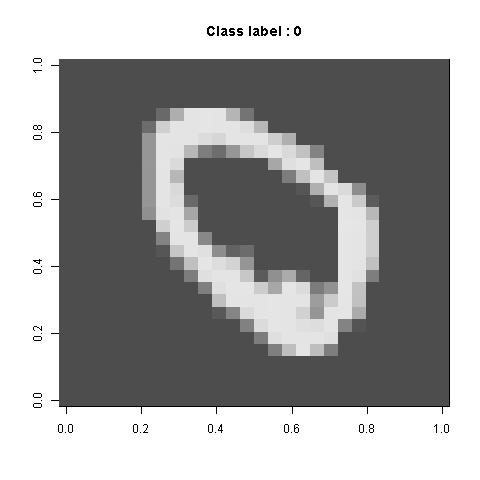
\includegraphics{0.jpg} \\
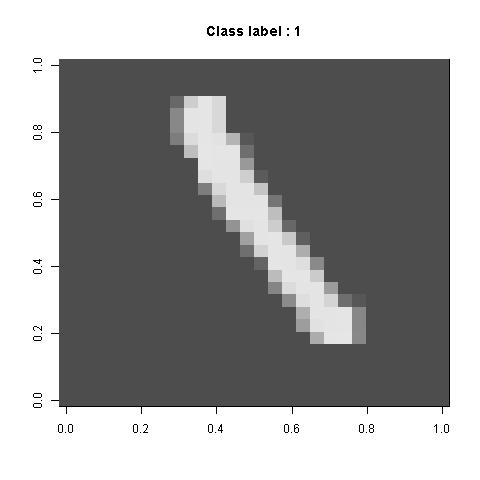
\includegraphics{1.jpg} \\
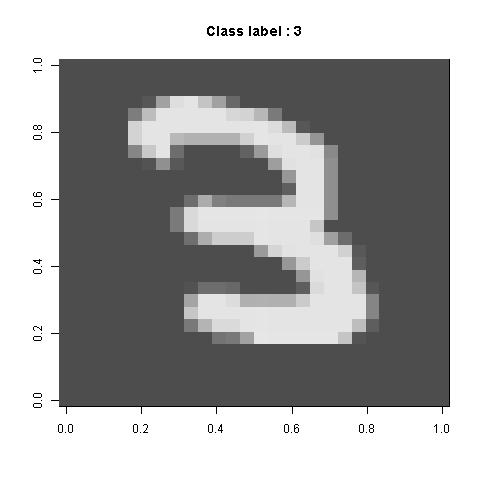
\includegraphics{3.jpg} \\
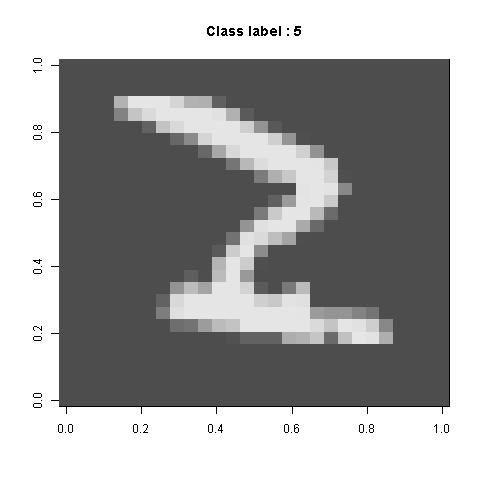
\includegraphics{5.jpg} \\

\setcounter{secnumdepth}{1}

\section{Theory}

\textbf{a} Write down the formula for computing the gradient of the loss function used in Logistic Regression. Specify what each variable represents in the equation.\\

The formula for the gradient descent is:
\[
\theta_j \leftarrow \theta_j - \alpha \sum_{i=1}^{n} \frac{1}{1 + \exp(-y^{(i)} <\theta, x^{(i)}> )}
\]
where $x^{(i)}$ is the data point represented in a vector of features, $y^{(i)}$ is the class label, and $\theta$ is the parameter vector. The goal is to reach the $\theta$ that maximizes our likelihood function (given the data we use to train the model).\\

\textbf{b} Write pseudocode for training a model using Logistic Regression.\\

\SetEndCharOfAlgoLine{}

\begin{algorithm}[H]
 \KwData{Training data}
 convergence threshold: $\eta$\;
 step size: $\alpha$\;
 \For{$j\leftarrow 0$ \KwTo $d$}{
  initialize $\theta_j$\;
  initialize $\Delta\theta_j$\;
 }
 
  \For{$i\leftarrow 1$ \KwTo $n$}{
  $x_0^{(i)} = 1$\;
 }
 \While{$\cup_{j\in\{0,1,...,d\}}|\delta\theta_j/\theta_j|>\eta$}{
    \For{$i\leftarrow 1$ \KwTo $n$}{
      $z^{(i)} = \sum_{j=0}^{d} \theta_j x_j^{(i)} $\;
      }
    \For{$j\leftarrow 0$ \KwTo $d$}{
      $\Delta = 0$\;
        \For{$i\leftarrow 1$ \KwTo $n$}{
            $\Delta \leftarrow \Delta + \frac{y^{(i)} x_j^{(i)}}{1 + \exp(-y^{(i)} z^{(i)} )}$\;
          }
      }
      $\theta_j \leftarrow $\theta_j - \alpha\Delta$\;
      $\delta\theta_j = \alpha\Delta$\;
 }
  \Return $\{\theta_0,...,\theta_d\}$\;
\end{algorithm}\DecMargin{1em}

\textbf{c} Calculate the number of operations per gradient descent iteration.\\
Each gradient descent update iteration requires $2n(d + 1)$\\

\section{Implementation}
\begin{Schunk}
\begin{Sinput}
> # Gredient Descent
> gradient_descent <- function(X, Y, XY, theta){
+     z <- as.matrix(X) %*% theta
+     yz_exp <- 1 / (1 + exp(-Y * z))
+     # Precalculate that instead for performance
+     #tmp <- apply(X,2,function(x) X * Y)
+     delta_theta <- t(XY) %*% yz_exp
+     return(delta_theta)
+ }
> # Logistic Regression
> # threshold should be higher than 100 but I used 100 by default to speed up the calculations need for the report
> logistic_regression <- function(X, Y, deviation, alpha, eta, seed = 100, threshold = 100) {
+   # initializations
+   set.seed(seed)
+   X$intercept <- 1
+   theta <- rnorm(ncol(X), sd = deviation)
+   delta_theta <- rep(10000, ncol(X))
+   numIterations <- 1
+   
+   #XY <- apply(X,2,function(x) X * Y)
+   XY <- sweep(X, 1,Y, "*")
+   while (any(abs(alpha * delta_theta/(theta + 0.0001)) > eta) & numIterations < threshold){
+     delta_theta <- gradient_descent(X,Y, XY,theta)
+     theta <- theta - alpha * delta_theta
+     numIterations <- numIterations + 1
+   }
+   return(theta)
+ }
\end{Sinput}
\end{Schunk}

\section{Training}
\textbf{a} Train 2 models, one on the train_0_1 set and another on train_3_5, and report the\\
training and test accuracies.
\begin{Schunk}
\begin{Sinput}
> # Calculate the predictions
> predict <- function(thetasFromTraining, classLabel){
+   classLabel$intercept <- 1
+   -sign(as.matrix(classLabel) %*% thetasFromTraining)
+ }
> # Calculate the accuracy
> accuracy <- function(model_function, X, Y, deviation, alpha = 0.001, eta = 0.000001, seed = 100, threshold = 100){
+   model_output <- model_function(X, Y, deviation, alpha, eta, seed, threshold)
+   a <- predict(model_output, X)
+   tmp <- mean(Y == a)
+   return(tmp)
+ }
> theta <- rnorm(ncol(train_0_1), sd = 0.5)
> accuracy(logistic_regression, train_0_1, true_label_train_0_1, deviation = 0.5)
\end{Sinput}
\begin{Soutput}
[1] 0.5323332
\end{Soutput}
\begin{Sinput}
> accuracy(logistic_regression, train_3_5, true_label_train_3_5, deviation = 0.5)
\end{Sinput}
\begin{Soutput}
[1] 0
\end{Soutput}
\end{Schunk}

\textbf{b} Repeat 3a 10 times, i.e. you should obtain 10 train and test accuracies for each set.
Calculate the average train and test accuracies over the 10 runs, and report them.

\begin{Schunk}
\begin{Sinput}
> train_0_1_accuracies <- numeric()
> for(i in 1:10){ 
+   train_0_1_accuracies <- append(train_0_1_accuracies, accuracy(logistic_regression, train_0_1, true_label_train_0_1, deviation = 0.5 ))
+ }
> mean(train_0_1_accuracies)
\end{Sinput}
\begin{Soutput}
[1] 0.5323332
\end{Soutput}
\begin{Sinput}
> train_3_5_accuracies <- numeric()
> for(i in 1:10){ 
+   train_3_5_accuracies <- append(train_3_5_accuracies, accuracy(logistic_regression, train_3_5, true_label_train_3_5, deviation = 0.5))
+ }
> mean(train_3_5_accuracies)
\end{Sinput}
\begin{Soutput}
[1] 0
\end{Soutput}
\begin{Sinput}
> test_0_1_accuracies <- numeric()
> for(i in 1:10){
+  test_0_1_accuracies <- append(test_0_1_accuracies, accuracy(logistic_regression, test_0_1, true_label_test_0_1, deviation = 0.5)) 
+ }
> mean(test_0_1_accuracies)
\end{Sinput}
\begin{Soutput}
[1] 0.536643
\end{Soutput}
\begin{Sinput}
> test_3_5_accuracies <- numeric()
> for(i in 1:10){
+   test_3_5_accuracies <- append(test_3_5_accuracies, accuracy(logistic_regression, test_3_5, true_label_test_3_5, deviation = 0.5))
+ }
> mean(test_3_5_accuracies)
\end{Sinput}
\begin{Soutput}
[1] 0
\end{Soutput}
\begin{Sinput}
> 
\end{Sinput}
\end{Schunk}

\textbf{c} For 0,1 and 3,5 cases, explain if you�observe any difference you in accuracy. Also,\\
explain why do you think this difference might be.\\

\textbf{d} This assignment deals with binary classification. Explain what you would do if you \\
had more than two classes to classify, using logistic regression.\\
Since logistic regression can only classify into two classes, I will use N-1 logistic regression\\ 
models where N is the number of outcome classes we have. Each model $m_i$ will classify  each un-classified \\
observation into two outcomes: wether the observation falls in class $n_i$ or not. By running these models \\
in sequence, the number of un-classified observations will get reduced untill we have all observations \\
getting classified by one of the models, or remain un-classified.

\section{Evaluation}

\textbf{a} Experiment with different initializations of the parameter used for gradient descent�\\
Clearly mention the initial values of the parameter tried, run the same experiment \\
as 3b using this initialization, report the average test and train accuracies obtained \\
by using this initialization, mention which is set of initializations is the better.\\

\textbf{initial_parameters_baseline} : 

\begin{itemize}
  \item theta = rnorm(ncol(train_0_1), sd = 0.5)
  \item alpha = 0.001
  \item eta = 0.000001
  \item threshold = 100 (Threshold should be higher than 100 but I used 100 by default to speed up the calculations needed for the report.)
\end{itemize}

\textbf{convergence_criteria_baseline} : (abs(alpha * delta_theta/(theta + 0.0001)) > eta) OR (numIterations < threshold) \\

Changing the initial parameters and keeping the convergence criteria the same. I obtained a new initial theta by changing the standard deviation I used for generating it.

\begin{Schunk}
\begin{Sinput}
> train_0_1_accuracies <- numeric()
> t <- rnorm(ncol(train_0_1), sd = 0.7)
> for(i in 1:10){ 
+   train_0_1_accuracies <- append(train_0_1_accuracies, 
+                                  accuracy(logistic_regression, 
+                                           train_0_1, true_label_train_0_1, 
+                                           theta = t
+                                           )
+                                  )
+ }


\end{document}
